% Prof. Dr. Ausberto S. Castro Vera
% UENF - CCT - LCMAT - Curso de Ci\^{e}ncia da Computa\c{c}\~{a}o
% Campos, RJ,  2023
% Disciplina: Paradigmas de Linguagens de Programa\c{c}\~{a}o
% Aluno: Gabriel Costa Fassarella



\chapterimage{ScalaH} % Chapter heading image ==>  Trocar este arquivo por outro 1200x468
\chapter{Ferramentas existentes e utilizadas}

Neste capítulo serão apresentadas duas ferramentas que foram utilizadas no desenvolvimento desse livro, e que também podem ser usadas pelo leitor. São elas: o Visual Studio Code (VS Code) e o Scastie.
\begin{itemize}
  \item Nome da ferramenta (compilador-interpretador)
  \item Endere\c{c}o na Internet
  \item Vers\~{a}o atual e utilizada
  \item Descri\c{c}\~{a}o simples (m\'{a}x 2 par\'{a}grafos)
  \item Telas capturadas da ferramenta
  \item Outras informa\c{c}\~{o}es
\end{itemize}


    \section{Visual Studio Code (VS Code)}
	Segundo \cite{Plainer}, o Visual Studio Code, ou simplesmente VS Code, é uma IDE desenvolvida pela Microsoft. Ela é um ambiente de programação gratuito e de código aberto que possui o suporte para inúmeras linguagens de programação diferentes e que pode ser executada em diversos sistemas operacionais, como o Windows, macOS ou Linux.
	
	Uma das principais características do VS Code é apresentar uma interface gráfica extremamente leve e personalizável, além disso a IDE fornece ao usuário uma diversa quantia de recursos como extensões que podem ser instaladas fornecendo ao usuário uma ampla gama de possibilidades. Isso faz com que a IDE suporte várias linguagens de programação diferentes, e para que a IDE rode códigos em Scala, é necessário duas extensões diferentes, a primeira o Scala Syntax e o Scala Metals, e além disso é necessário compilar os códigos na linguagem, para isso deve-se instalar a extensão Code runner. Vale lembrar que durante o desenvolvimento desse livro, foi utilizada a IDE na versão 1.79.1.
	
	A IDE pode ser instalada em sua atual versão \href{https://code.visualstudio.com}{aqui}.

	Imagens da ferramenta com a implementação de alguns códigos simples:
	
	\begin{figure}[H]
		\centering
		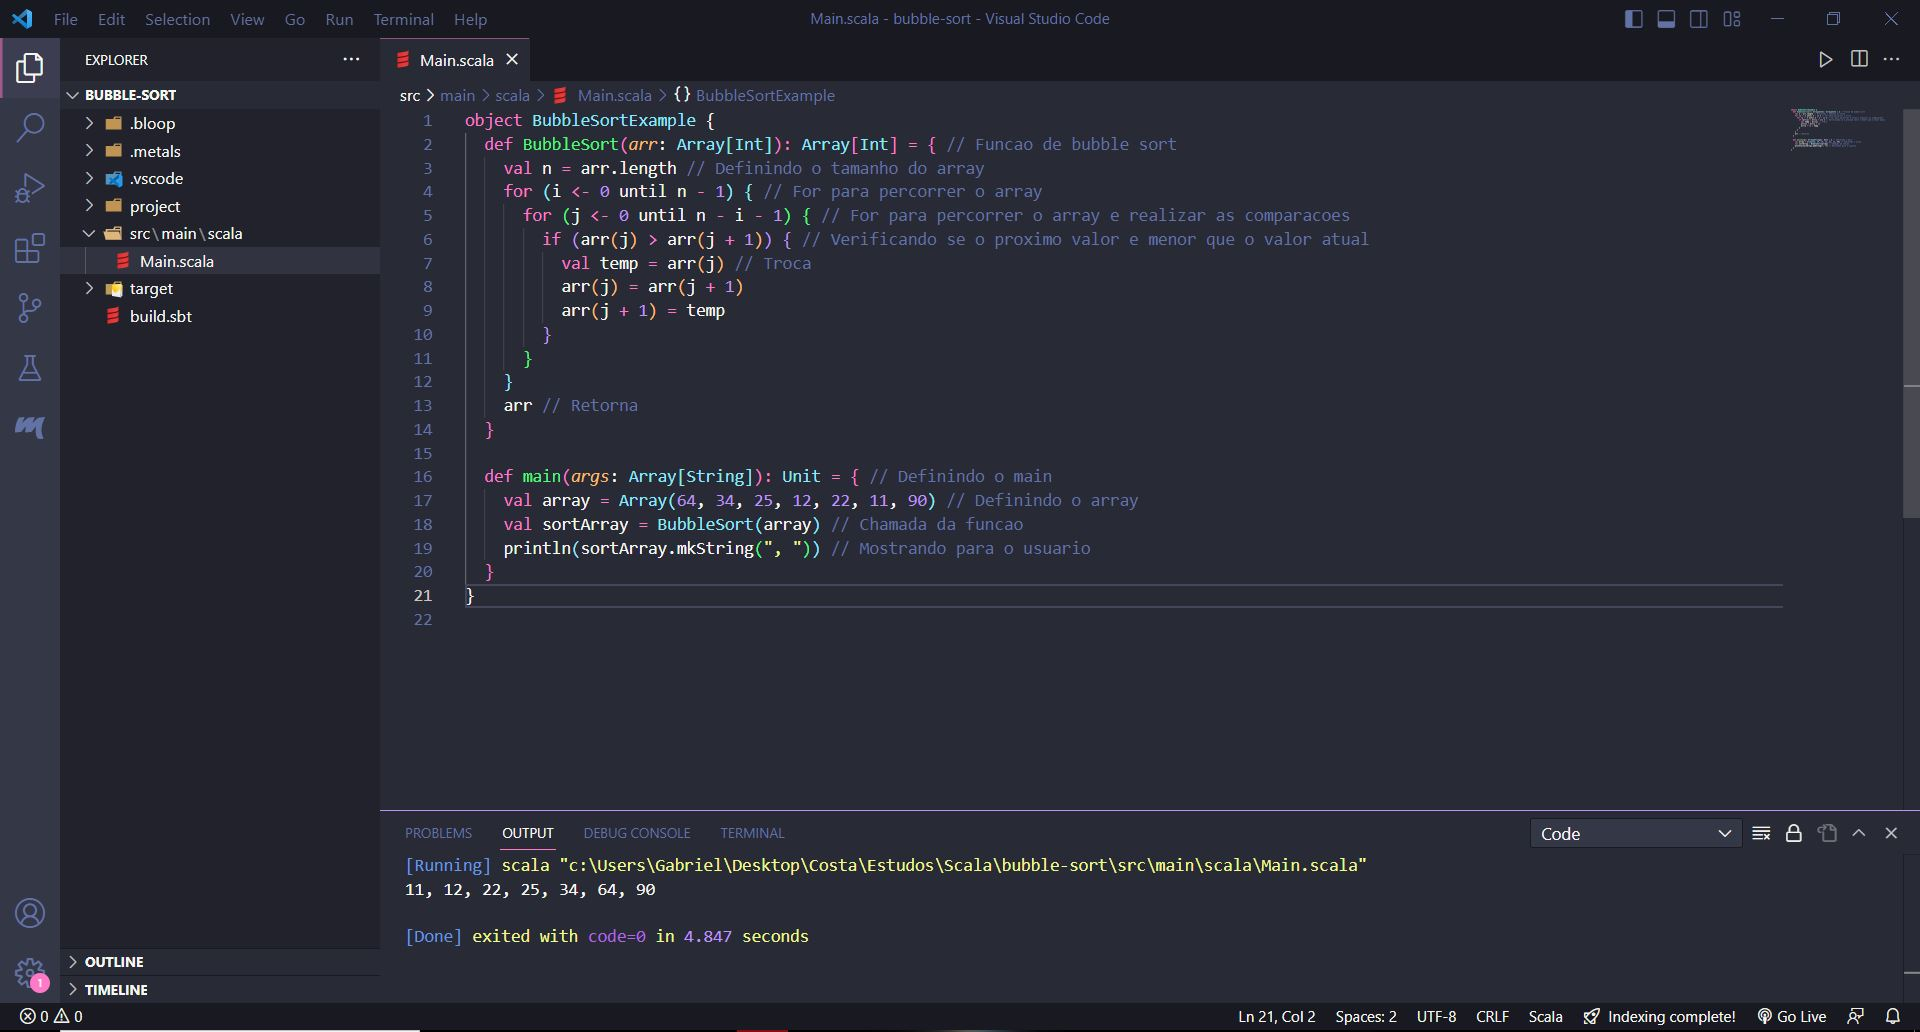
\includegraphics[width=17.5cm]{Pictures/Ferr1.1.jpg}
		\caption{}
		\label{fig:ferr1}
	\end{figure}
	
	\begin{figure}[H]
		\centering
		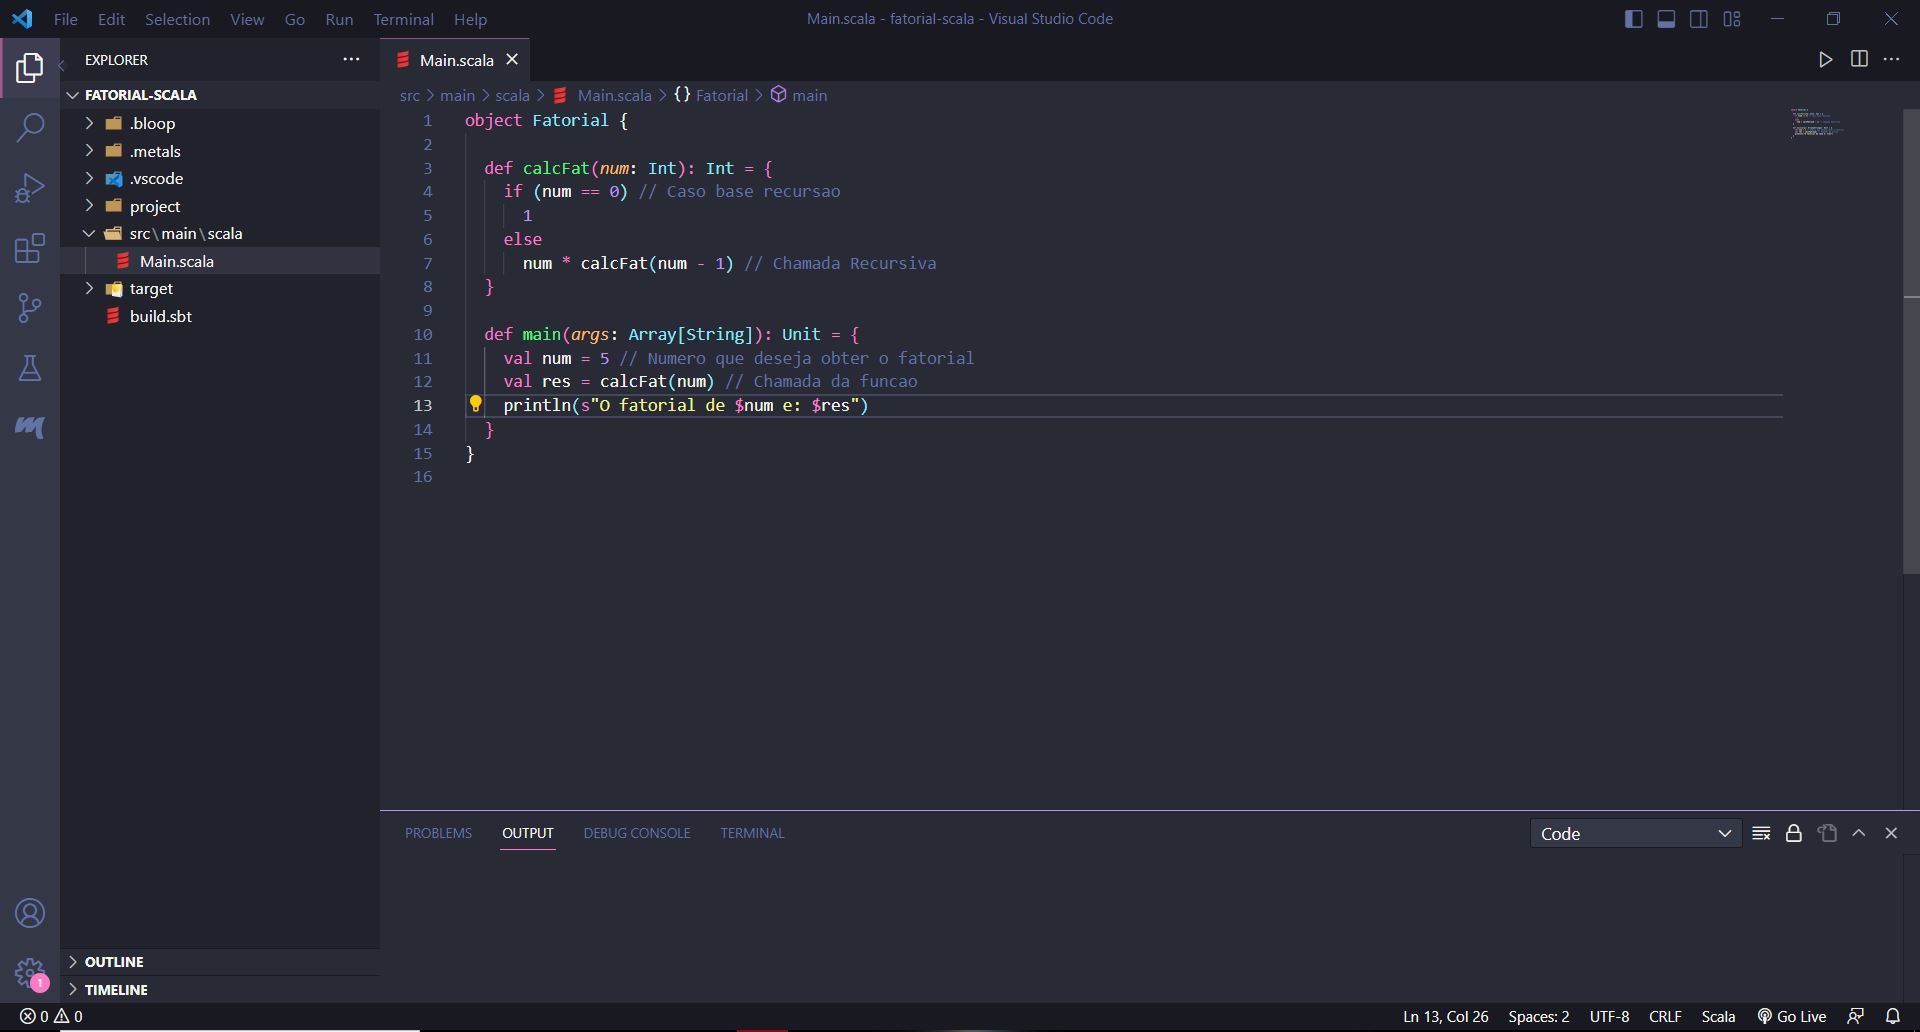
\includegraphics[width=17.5cm]{Pictures/Ferr1.2.jpg}
		\caption{}
		\label{fig:ferr2}
	\end{figure}

	\begin{figure}[H]
		\centering
		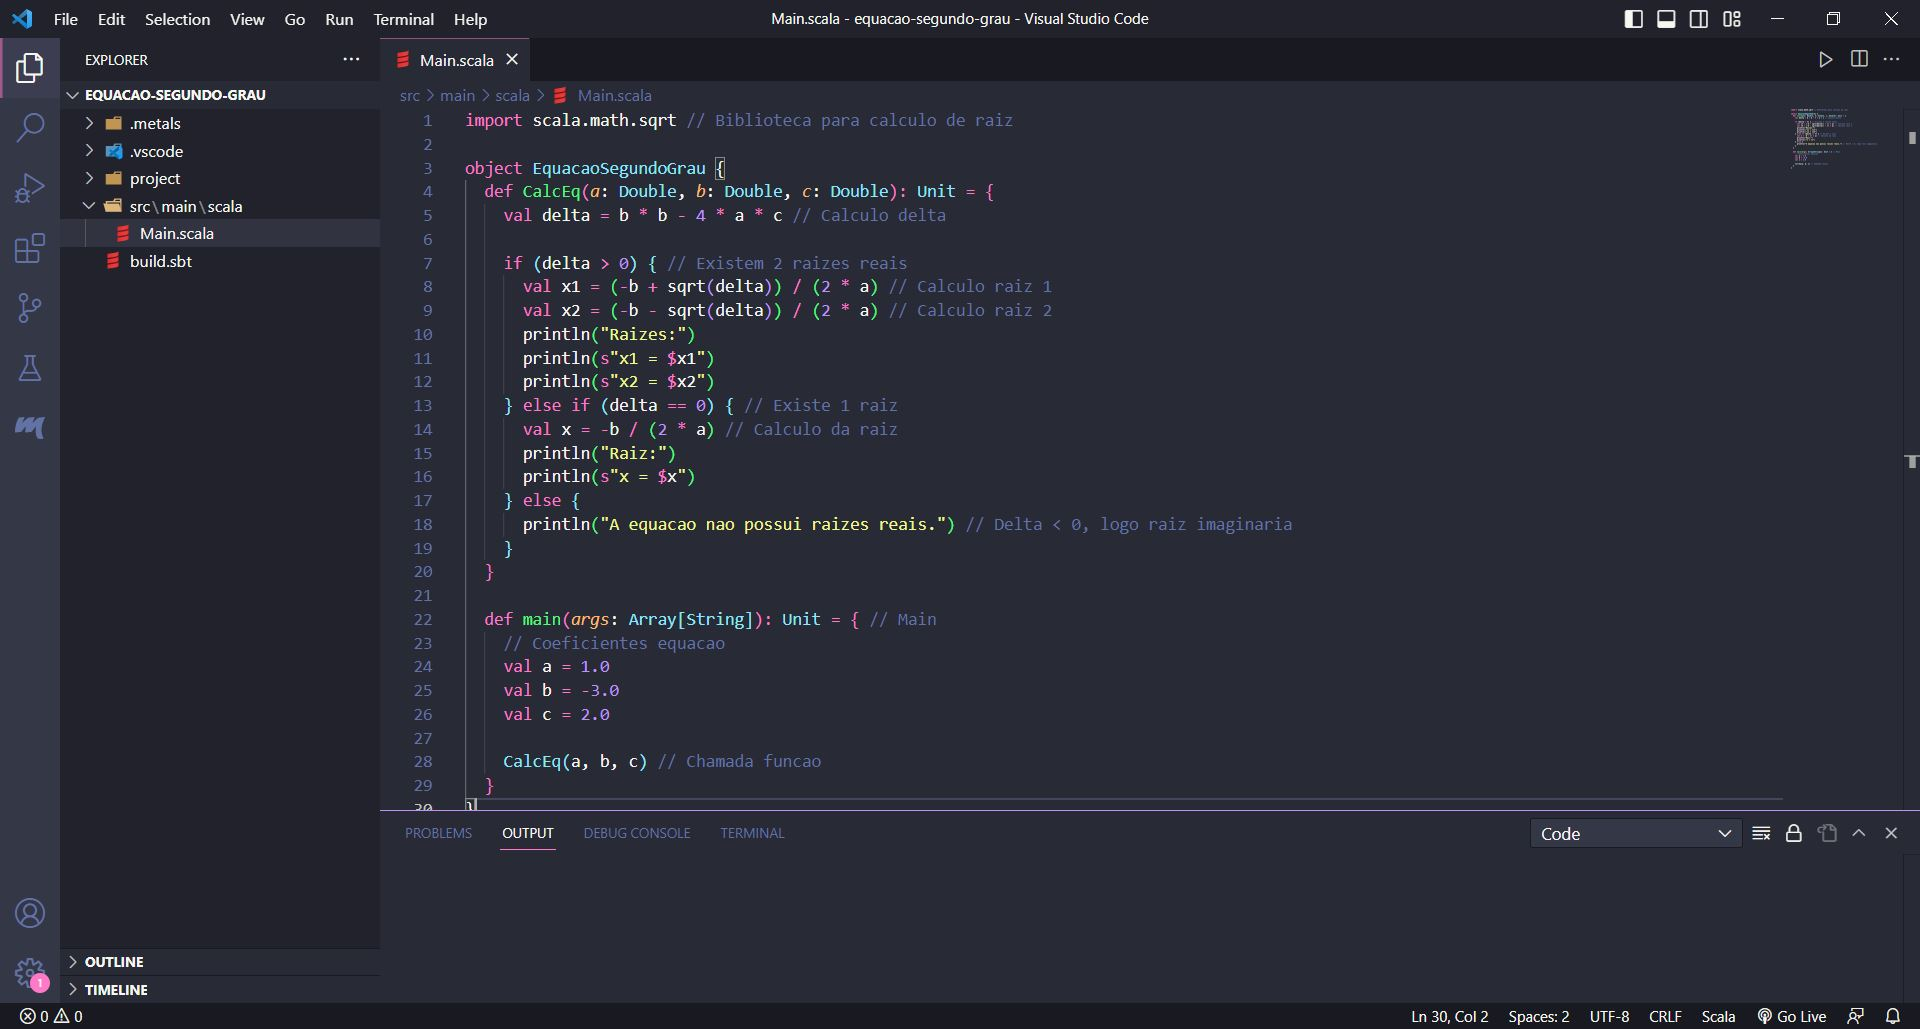
\includegraphics[width=17.5cm]{Pictures/Ferr1.3.jpg}
		\caption{}
		\label{fig:ferr3}
	\end{figure}

	Imagem da aba de extensões do VS Code: 
	\begin{figure}[H]
		\centering
		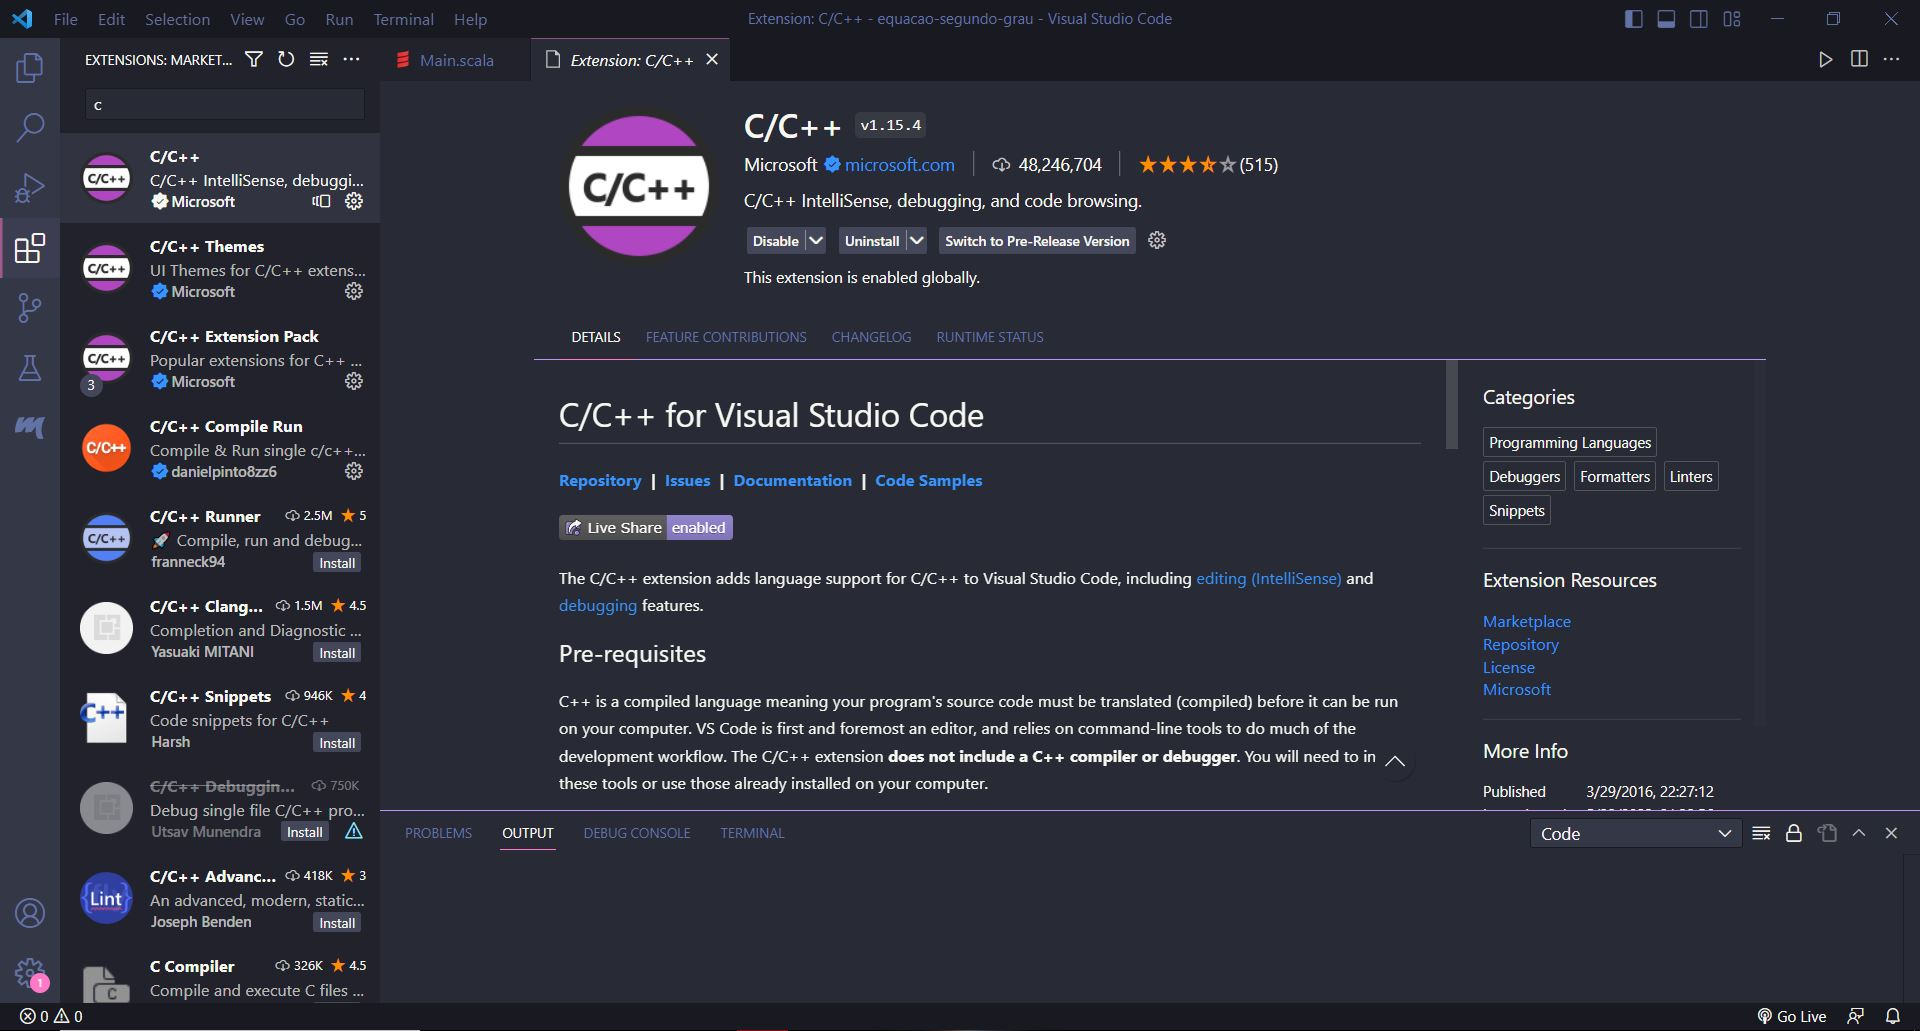
\includegraphics[width=17.5cm]{Pictures/Ferr1.4.jpg}
		\caption{}
		\label{fig:ferr4}
	\end{figure}
	

    \section{Scastie}
    O Scastie é uma plataforma online que permite executar código em Scala. É um ambiente de programação baseado na web criado com o intuito de ser de fácil acesso e interativo, e com o principal propósito: não precisar instalar nenhum software.
    
    Uma das características mais notáveis do Scastie é a capacidade de compartilhar códigos com outros usuários, facilitando a colaboração de diferentes programadores. Além disso, o ambiente de programação possibilita o usuário importar bibliotecas. Isso faz com que o Scastie seja uma ótima ferramenta para pessoas que desejam estudar, testar e compartilhar códigos em Scala.
    
    A ferramenta pode ser encontrada no próprio site do Scala ou clicando \href{https://scastie.scala-lang.org}{aqui}.
    
    \begin{figure}[H]
    	\centering
    	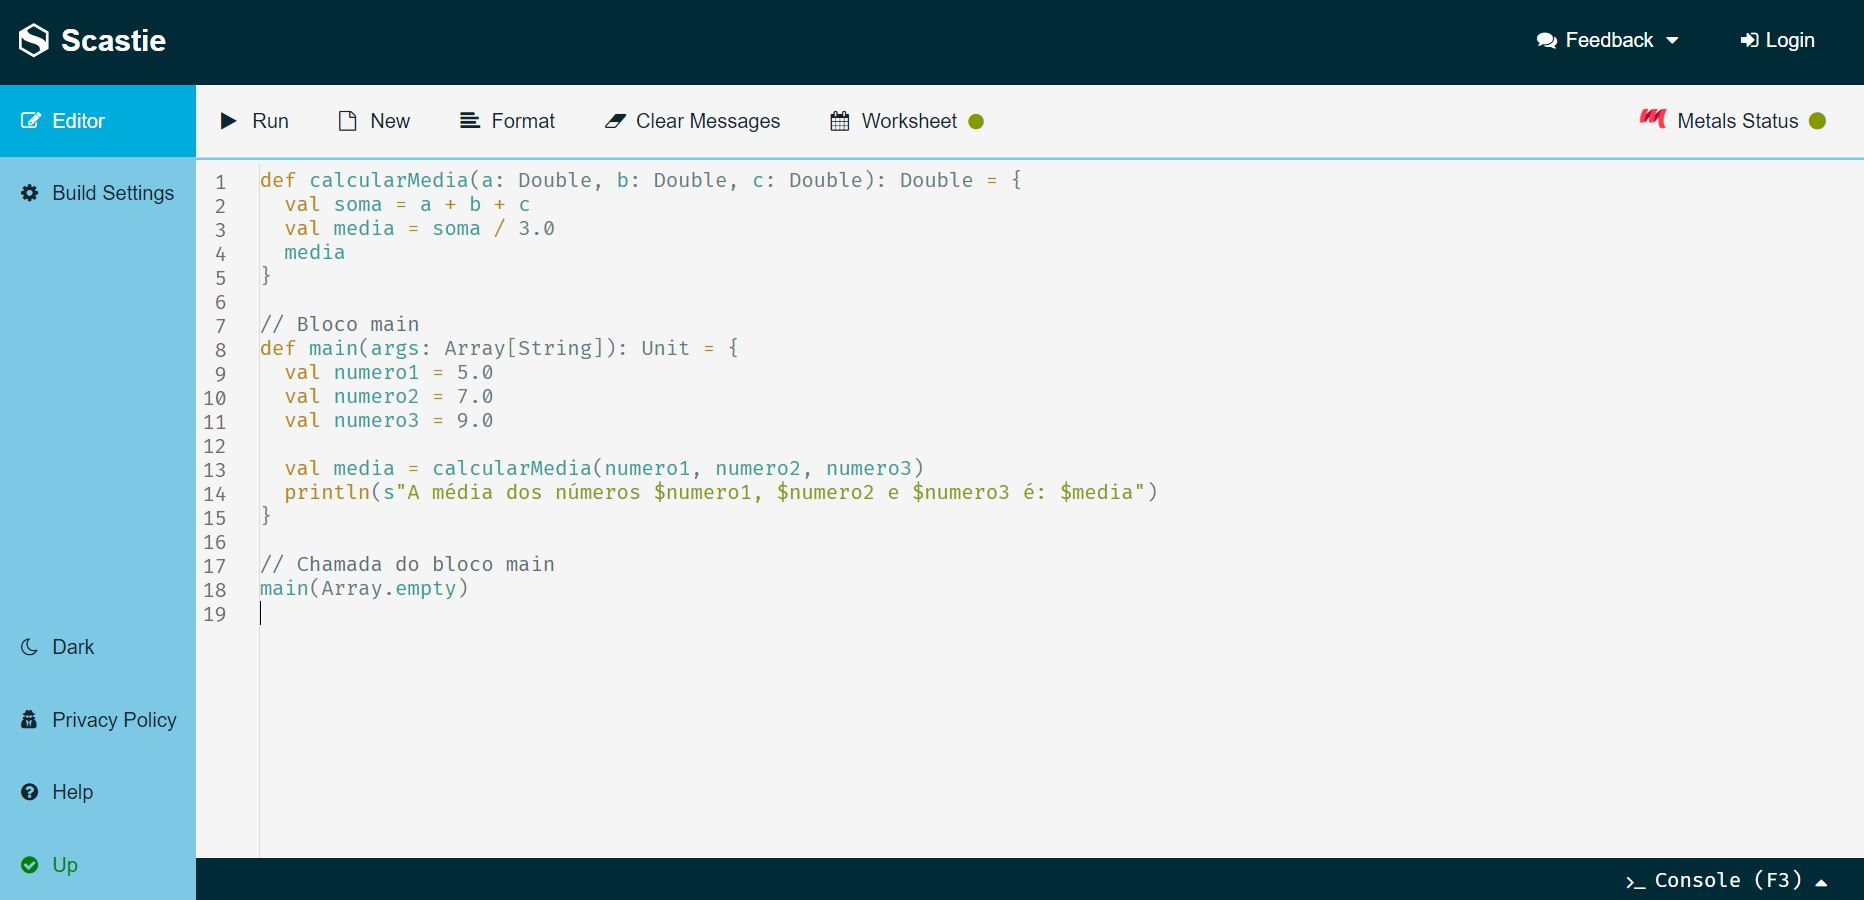
\includegraphics[width=17.5cm]{Pictures/Ferr2.1.jpg}
    	\caption{}
    	\label{fig:ferr1}
    \end{figure}

    \begin{figure}[H]
		\centering
		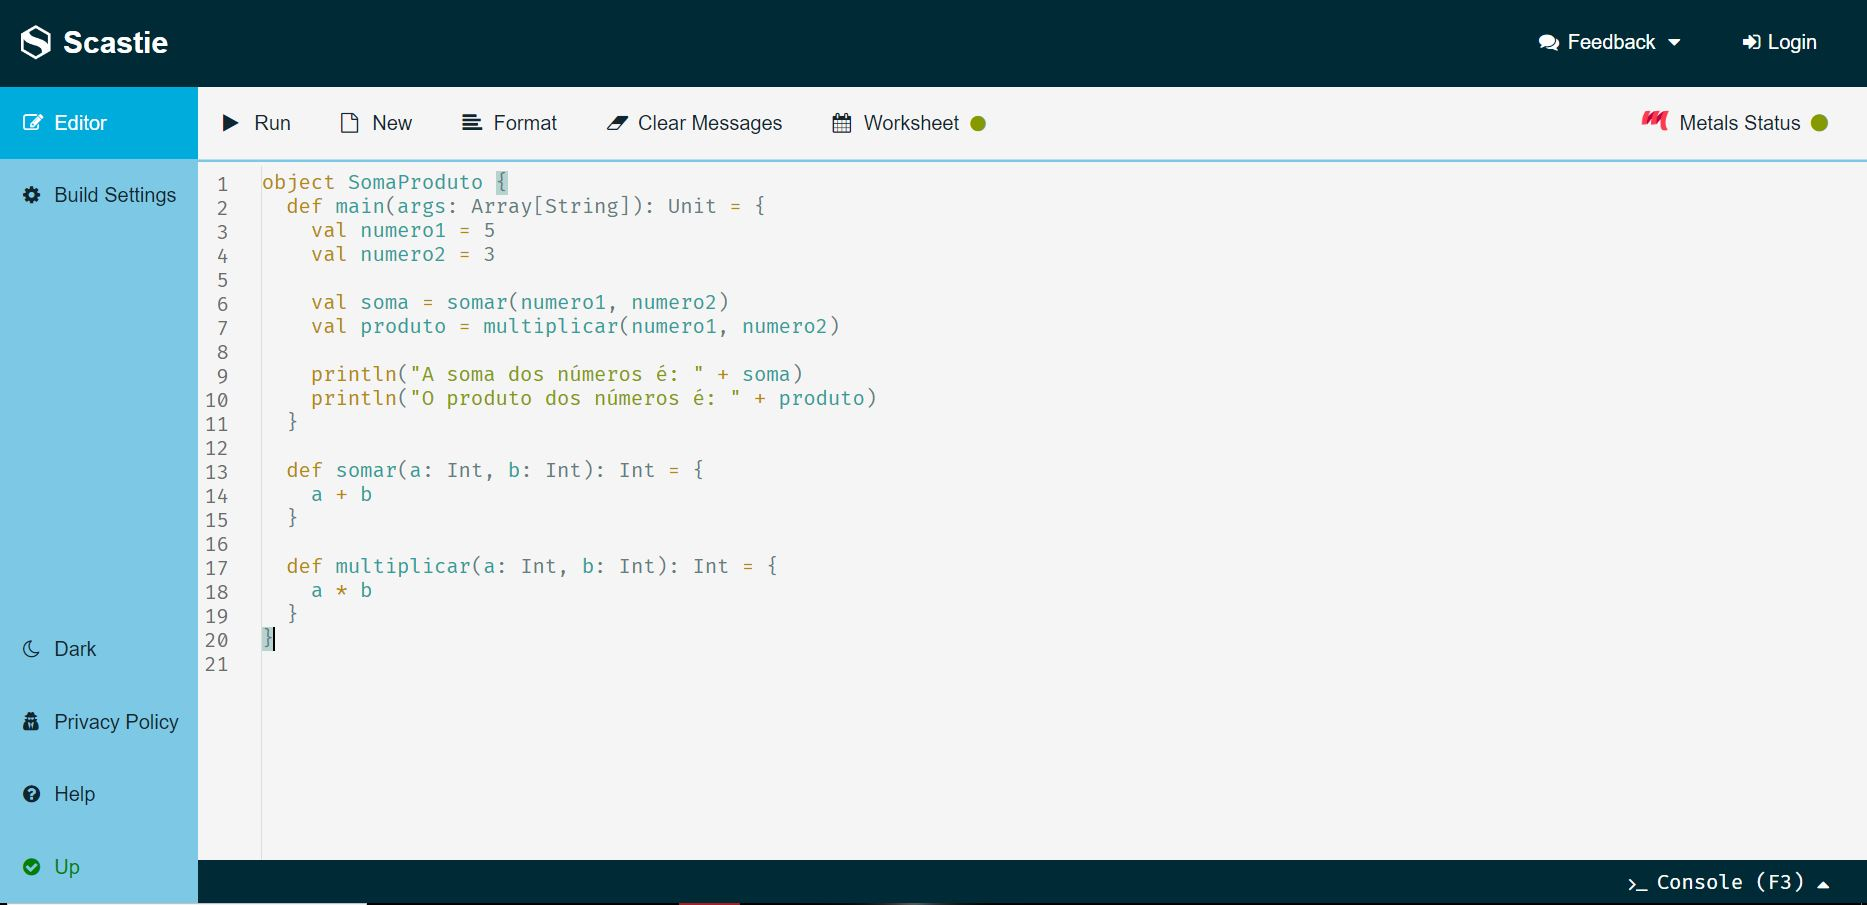
\includegraphics[width=17.5cm]{Pictures/Ferr2.2.jpg}
		\caption{}
		\label{fig:ferr2}
	\end{figure}

	\begin{figure}[H]
		\centering
		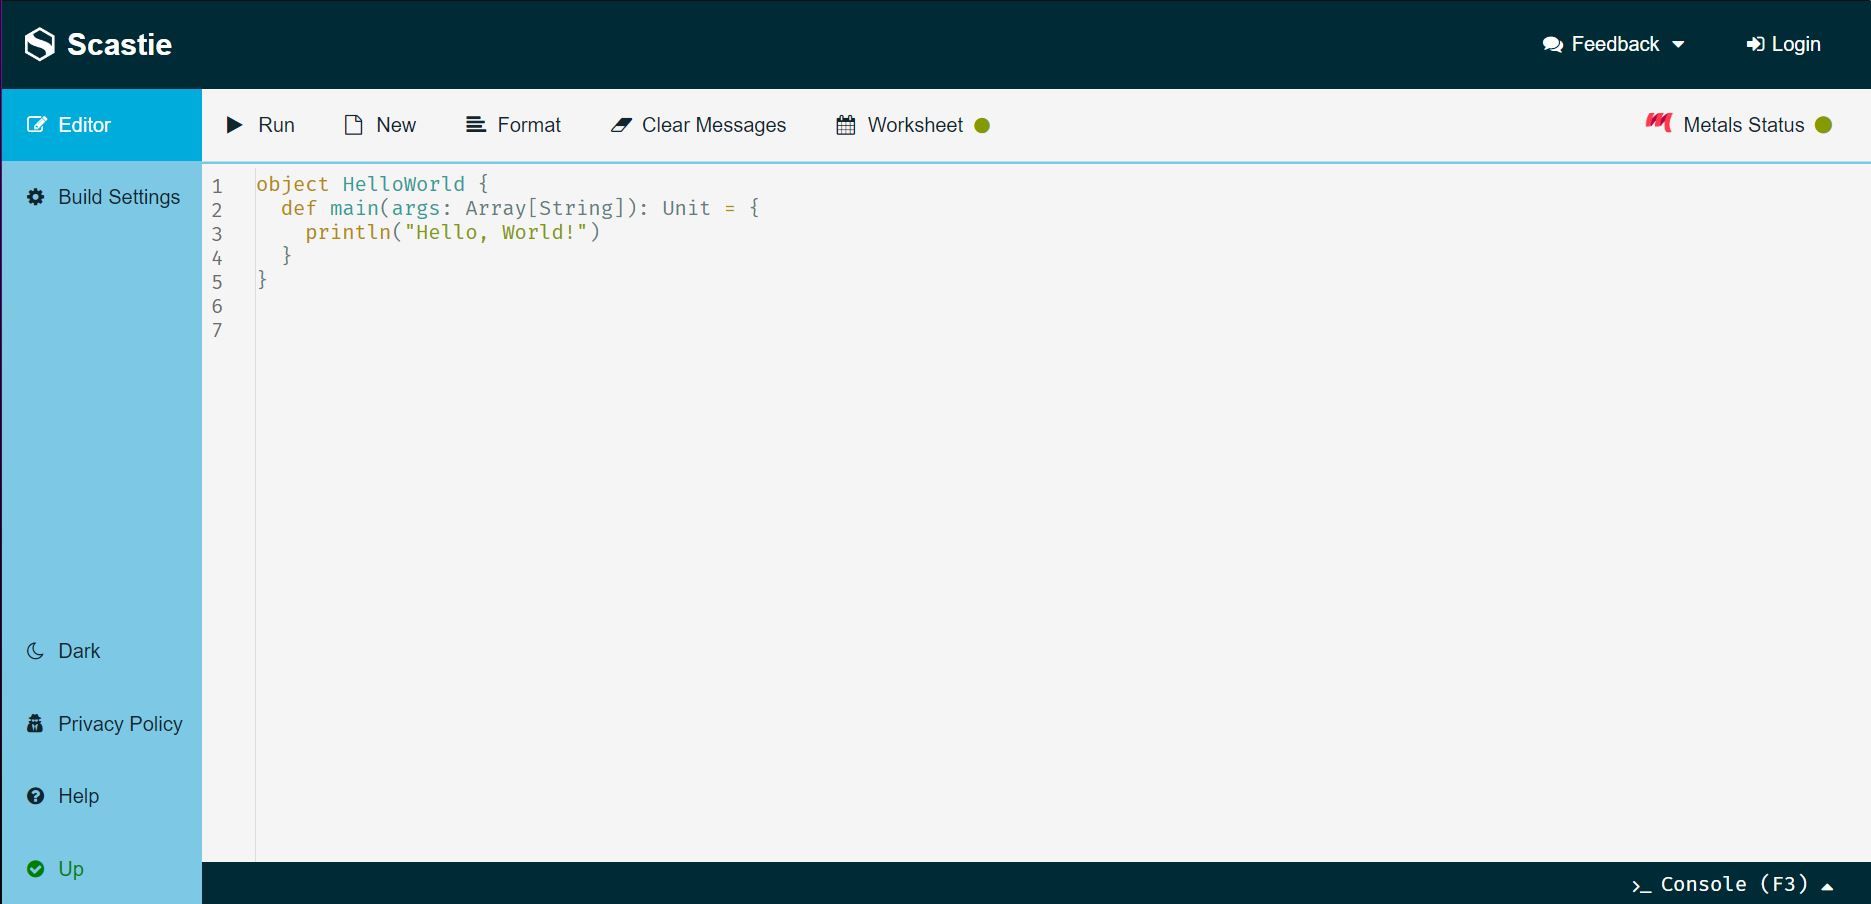
\includegraphics[width=17.5cm]{Pictures/Ferr2.3.jpg}
		\caption{}
		\label{fig:ferr3}
	\end{figure}
